\documentclass[11pt]{standalone}
\usepackage[T1]{fontenc}
\usepackage{tikz}
\usetikzlibrary{calc,positioning,shapes.geometric}

\begin{document}
  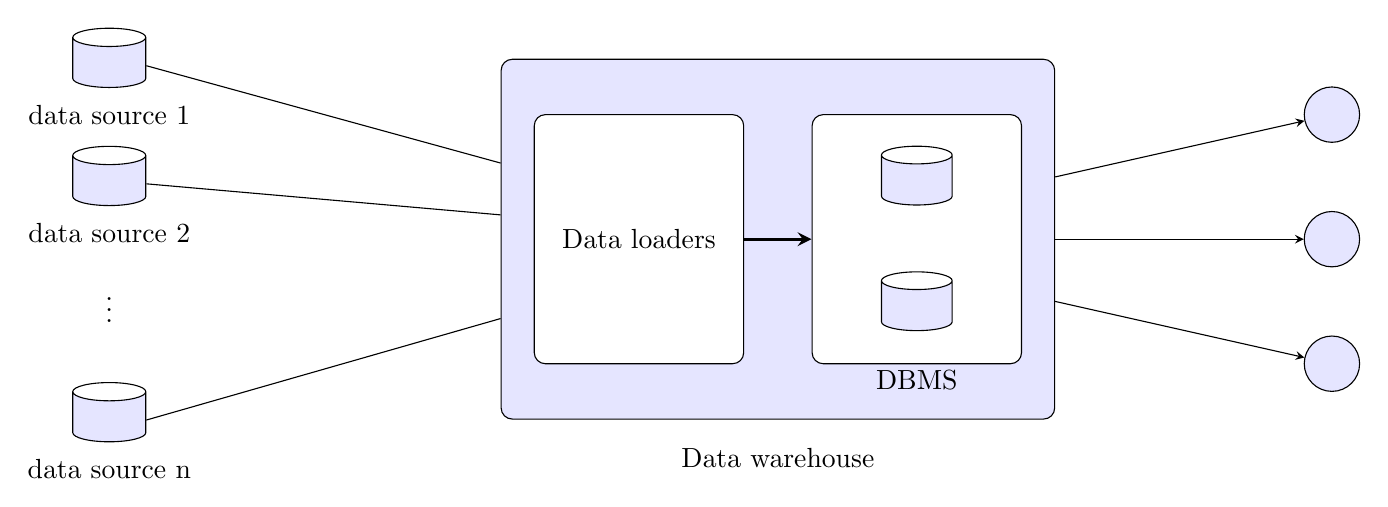
\begin{tikzpicture}[
    >=stealth,
    node distance=1.5cm,
    database/.style={
      cylinder,
      text opacity=0,
      cylinder uses custom fill,
      cylinder body fill=blue!10,
      cylinder end fill=white!50,
      shape border rotate=90,
      aspect=0.25,
      draw
    }
  ]
    \node[database, label={[anchor=north, inner sep=0pt, yshift=-0.6em, text=black]south:data source 1}] (db1) at (0,0) {DB1};
    \node[database, label={[anchor=north, inner sep=0pt, yshift=-0.6em, text=black]south:data source 2}, below of=db1] (db2) {DB2};
    \node[below of=db2] (dbDots) {$\vdots$};
    \node[database, label={[anchor=north, inner sep=0pt, yshift=-0.6em, text=black]south:data source n}, below of=dbDots] (db3) {DB3};

    % THEME BLOCK 
    \node[rounded corners, %fill=black,
    text depth = 5em,
    draw,
    % double distance =1pt,    %% here
    %font=\Large, 
    minimum height= 13em,
    minimum width= 20em,
    fill=blue!10,
    label={[anchor=north, inner sep=0pt, yshift=-1em] south:{Data warehouse}}] at ([xshift=25.5em, yshift=-2em]
    db2.west) (dw){};
    
    % Configuration Files and Plugin box
    \node[rounded corners, %fill=black,
    draw,
    text centered,
    text width = 0.20\textwidth,
    fill=white,
    minimum height= 9em,
    minimum width= 2em] at ([xshift=5em] dw.west) (dl){Data loaders};
    \node[rounded corners, %fill=black,
    draw,
    text centered,
    text width = 0.20\textwidth,
    fill=white,
    minimum height= 9em,
    minimum width= 2em,
    label={[anchor=north, inner sep=0pt, yshift=-0.2em] south:{DBMS}}] at ([xshift=-5em] dw.east) (dbms){};
    \node[database] at ([yshift=-2.5em] dbms.north) {din1};
    \node[database] at ([yshift= 2em] dbms.south) {din2};
    
    
    \node[circle, fill=blue!10, draw, minimum width=2em] at ([xshift=10em] dw.east) (c2) {};
    \node[circle, fill=blue!10, draw, minimum width=2em] at ([yshift=4.5em, xshift=10em] dw.east) (c1) {};
    \node[circle, fill=blue!10, draw, minimum width=2em] at ([yshift=-4.5em, xshift=10em] dw.east) (c3) {};
    
    % arrows 
    
    \draw (db1.east) -- (dw);
    \draw (db2.east) -- (dw);
    \draw (db3.east) -- (dw);
    \draw[->] (dw) -> (c1);
    \draw[->] (dw) -> (c2);
    \draw[->] (dw) -> (c3);
    
    % Extra Thick arrow
    \draw[->, very thick] (dl) -> (dbms);
  \end{tikzpicture}
\end{document}